\documentclass{report}
    \title{\vspace{-50pt}\textbf{\underline{COP4620 Notes - Post-MidTerm}}}
    \author{William L. Thomson Jr.}
    \date{Spring Semester 2022}
    \usepackage{algorithm}
    \usepackage{algpseudocode}
    \usepackage{amsmath}
    \usepackage[dvipsnames]{xcolor}
    \usepackage{enumitem}
    \usepackage{helvet}
    \usepackage{hyperref}
    \usepackage{makecell}
    \usepackage{multicol}
    \usepackage{soul}
    \usepackage[T1]{fontenc}
    \usepackage{tikz}
    \usepackage[tmargin=1in,lmargin=1in,rmargin=1in]{geometry}
    \usepackage{titlesec}
    \usepackage{xcolor}
    \usetikzlibrary{automata, positioning, arrows, babel,positioning,shapes}

    \algdef{SE}{Begin}{End}{\textbf{begin}}{\textbf{end}}

    \hypersetup{ colorlinks=true, linkcolor=blue, filecolor=purple, urlcolor=cyan }

    \newcommand{\comment}[1]{}
    \newcommand{\textb}[1]{\textcolor{blue}{#1}}
    \newcommand{\textg}[1]{\textcolor{ForestGreen}{#1}}
    \newcommand{\textp}[1]{\textcolor{purple}{#1}}
    \newcommand{\textr}[1]{\textcolor{red}{#1}}
    \newcommand{\textbfb}[1]{\textbf{\textb{#1}}}
    \newcommand{\textbfg}[1]{\textbf{\textg{#1}}}
    \newcommand{\textbfp}[1]{\textbf{\textp{#1}}}
    \newcommand{\textbfr}[1]{\textbf{\textr{#1}}}

    \newlength\tindent
    \setlength{\tindent}{\parindent}
    \setlength{\parindent}{0pt}
    \renewcommand{\indent}{\hspace*{\tindent}}
    
    \renewcommand{\familydefault}{\sfdefault}

    \setlist[description]{noitemsep, topsep=0pt, itemsep=-.1em}
    \setlist[enumerate]{noitemsep, topsep=0pt, itemsep=-.1em}
    \setlist[itemize]{noitemsep, topsep=0pt, itemsep=-.1em}

	\titleformat{\chapter}[display]{\bfseries\Large\itshape}{Lecture - \thechapter}{0.5ex}{ }
	\titleformat{\section}{\normalfont\bfseries}{\thesection}{0.5em}{}
	\titleformat{\subsection}{\normalfont\bfseries}{\thesubsection}{0.5em}{}

    \titlespacing\chapter{0pt}{12pt plus 0pt minus 4pt}{0pt plus 0pt minus 4pt}
    \titlespacing\section{0pt}{12pt plus 4pt minus 8pt}{0pt plus 2pt minus 8pt}
    \titlespacing\subsection{0pt}{12pt plus 4pt minus 4pt}{0pt plus 2pt minus 4pt}
    \titlespacing\subsubsection{0pt}{12pt plus 4pt minus 2pt}{0pt plus 2pt minus 2pt}

    \tikzset{
        node distance=3cm, % minimum distance between two nodes. Change if necessary.
        every state/.style={thick, fill=gray!10}, % sets properties for each state node
        initial text=$ $, % sets the text that appears on the start arrow
    }
    \tikzset{
      gray box/.style={
		fill=gray!20,
		draw=gray,
		minimum width={2*#1ex},
		minimum height={2em},
	  },
  		annotation/.style={
    	anchor=north,
      }
  	}
    \tikzstyle{vertex}=[draw,fill=black!15,circle,minimum size=20pt,inner sep=0pt]

\begin{document}

\maketitle
\tableofcontents

\setcounter{chapter}{3}
\chapter{Semantic Actions for Declarations and Expressions}
\vspace{-1em}
\begin{multicols}{2}
\textbf{Grammar} \\
assign $\rightarrow$ ID := expr \\
expr   \hspace{.7em}$\rightarrow$ term addop term \\
term   \hspace{.6em}$\rightarrow$ ID | LIT \\
addop  $\rightarrow$ + | -
\vfill\columnbreak
\textbf{Annotated with Semantic Actions} \\
assign $\rightarrow$ ID \textr{\#process\_id} := exp \textr{\#gen\_assign} \\
expr   \hspace{.7em}$\rightarrow$ term addop term \textr{\#gen\_infix} \\
term   \hspace{.6em}$\rightarrow$ ID \textr{\#process\_id} | LIT \textr{\#process\_lit} \\
addop  $\rightarrow$  + \textr{\#process\_p} | - \textr{\#process\_m}
\end{multicols}
\vspace{-2em}


\section{In Class Quiz 1 - Slide 6}
Which sequence of actions are invoked for the string \textbfb{a := b + 1} \\
Replace expr, then replace terms, then replace addop
\begin{enumerate}
  \item assign $\rightarrow$ ID \textr{\#process\_id} := \textbf{exp} \textr{\#gen\_assign}
  \item assign $\rightarrow$ ID \textr{\#process\_id} := \textbf{term addop term} \textbfr{\#gen\_infix} \textr{\#gen\_assign}
  \item assign $\rightarrow$ ID \textr{\#process\_id} := \textbf{ID} \textbfr{\#process\_id} addop \textbf{LIT} \textbfr{\#process\_lit} \textr{\#gen\_infix} \textr{\#gen\_assign} 
  \item assign \hspace{.1em}$\rightarrow$ ID \textr{\#process\_id} := ID \textr{\#process\_id} \textbf{+} \textbfr{\#process\_p} LIT \textr{\#process\_lit} \textr{\#gen\_infix} \textr{\#gen\_assign} 
\end{enumerate}

Action sequence: \textbf{process\_id, process\_id, process\_op, process\_lit, gen\_infix, gen\_assign}
\vspace{-.5em}

\subsection{Semantic Stack}
\vspace{-1em}
\begin{multicols}{2}
  \begin{enumerate}
    \setlength{\leftskip}{-1.5em}
    \item \textbf{process\_id}  produces expression recognition for a
    \item \textbf{process\_id}  produces expression recognition for b
    \item \textbf{process\_p}   produces expression recognition for +
    \item \textbf{process\_lit} produces expression recognition for 1
    \item \textbf{gen\_infix} produces code (not final/intermediate)
     and a new expression record for b + 1
    \item \textbf{gen\_assign} produces code to assign b + 1 to a and clears the stack
  \end{enumerate}
\vfill\columnbreak
  \setlength{\leftskip}{2em}
  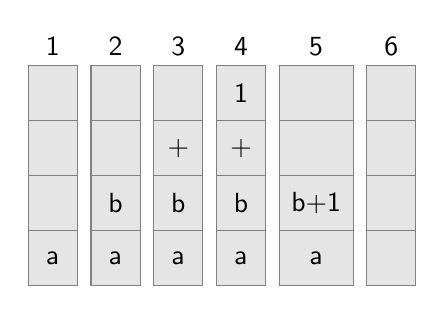
\begin{tikzpicture}[node distance=-0.5pt]
    \node [gray box=2] (10) {};
    \node [gray box=2, below=of 10] (11) {}; 
    \node [gray box=2, below=of 11] (12) {};
    \node [gray box=2, below=of 12] (13) {a};
    \node [gray box=2, right=of 10, xshift=5pt] (20) {};
    \node [gray box=2, below=of 20] (21) {}; 
    \node [gray box=2, below=of 21] (22) {b};
    \node [gray box=2, below=of 22] (23) {a};
    \node [gray box=2, right=of 20, xshift=5pt] (30) {};
    \node [gray box=2, below=of 30] (31) {+}; 
    \node [gray box=2, below=of 31] (32) {b};
    \node [gray box=2, below=of 32] (33) {a};
    \node [gray box=2, right=of 30, xshift=5pt] (40) {1};
    \node [gray box=2, below=of 40] (41) {+}; 
    \node [gray box=2, below=of 41] (42) {b};
    \node [gray box=2, below=of 42] (43) {a};
    \node [gray box=3, right=of 40, xshift=5pt] (50) {};
    \node [gray box=3, below=of 50] (51) {}; 
    \node [gray box=3, below=of 51] (52) {b+1};
    \node [gray box=3, below=of 52] (53) {a};
    \node [gray box=2, right=of 50, xshift=5pt] (60) {};
    \node [gray box=2, below=of 60] (61) {}; 
    \node [gray box=2, below=of 61] (62) {};
    \node [gray box=2, below=of 62] (63) {};
    \node [annotation, above] at (10.north) {1};
    \node [annotation, above] at (20.north) {2};
    \node [annotation, above] at (30.north) {3};
    \node [annotation, above] at (40.north) {4};
    \node [annotation, above] at (50.north) {5};
    \node [annotation, above] at (60.north) {6};
  \end{tikzpicture}
\end{multicols}
\vspace{-2.5em}

\section{In Class Quiz 2 - Slide 14}
Is the given scope stack correct for location D of the given code?  \textbf{Yes}
\vspace{-1em}
\begin{multicols}{2}
  \textb{
\vspace{-1em}
\begin{algorithmic}[1]
  \Begin
    \State declare H, A, L: integer; \textbfr{ $\leftarrow$ A}
    \Begin
      \Begin
        \State declare X, Y: Real; \textbfr{ $\leftarrow$ B}
      \End; \textbfr{ $\leftarrow$ C}
      \Begin
        \State declare A, C, M: char; \textbfr{ $\leftarrow$ D}
      \End;
    \End;
  \End;
\end{algorithmic}
  }
  \vfill\columnbreak
  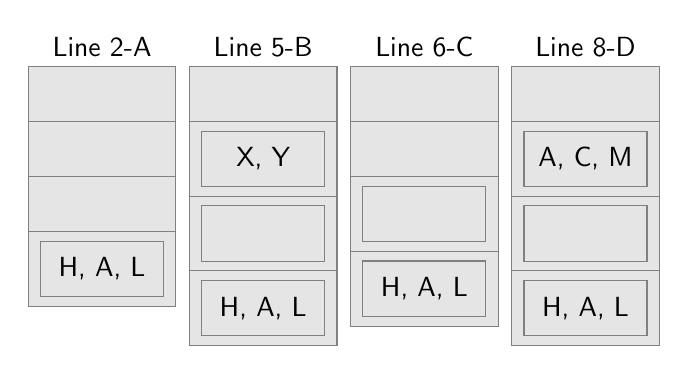
\begin{tikzpicture}[node distance=-0.5pt]
    \node [gray box=6] (10) {};
    \node [gray box=6, below=of 10] (11) {}; 
    \node [gray box=6, below=of 11] (12) {};
    \node [gray box=6, below=of 12] (13) {\tikz{\node[gray box=5] {H, A, L};}};
    \node [gray box=6, right=of 10, xshift=5pt] (20) {};
    \node [gray box=6, below=of 20] (21) {\tikz{\node[gray box=5] {X, Y};}}; 
    \node [gray box=6, below=of 21] (22) {\tikz{\node[gray box=5] {};}};
    \node [gray box=6, below=of 22] (23) {\tikz{\node[gray box=5] {H, A, L};}};
    \node [gray box=6, right=of 20, xshift=5pt] (30) {};
    \node [gray box=6, below=of 30] (31) {}; 
    \node [gray box=6, below=of 31] (32) {\tikz{\node[gray box=5] {};}};
    \node [gray box=6, below=of 32] (33) {\tikz{\node[gray box=5] {H, A, L};}};
    \node [gray box=6, right=of 30, xshift=5pt] (40) {};
    \node [gray box=6, below=of 40] (41) {\tikz{\node[gray box=5] {A, C, M};}}; 
    \node [gray box=6, below=of 41] (42) {\tikz{\node[gray box=5] {};}};
    \node [gray box=6, below=of 42] (43) {\tikz{\node[gray box=5] {H, A, L};}};
    \node [annotation, above] at (10.north) {Line 2-A};
    \node [annotation, above] at (20.north) {Line 5-B};
    \node [annotation, above] at (30.north) {Line 6-C};
    \node [annotation, above] at (40.north) {Line 8-D};
  \end{tikzpicture}
\end{multicols}
\vspace{-2em}


\section{In Class Quiz 3 - Slide 19}
Which sequence of actions are invoked for the string: \textbfb{INT a;} \\
var\_decl $\rightarrow$ var\_type id; \textr{\#decl\_id} \\
var\_type $\rightarrow$ INT \textr{\#int\_type} | FLOAT \textr{\#float\_type} \\
id $\rightarrow$ IDENTIFIER \textr{\#id} \\
Action sequence: \textbf{\#int\_type,\#id, \#decl\_id}
\vspace{-1em}
\begin{multicols}{2}
\begin{enumerate}
  \item int\_type() generate a record for "int"
  \item id() generates a record for "a"
  \item decl\_id() pop the two top most records \\
  and invokes ex $\rightarrow$ insert\_entry(int, a) \\
  if not in table add it, if already in table $\rightarrow$ error
\end{enumerate}
  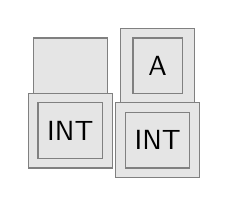
\begin{tikzpicture}[node distance=-0.5pt]
    \node [gray box=3] (10) {};
    \node [gray box=3, below=of 10] (11) {\tikz{\node[gray box=2] {INT};}};
    \node [gray box=3, right=of 10, xshift=5pt] (20) {\tikz{\node[gray box=2] {A};}};
    \node [gray box=3, below=of 20] (21) {\tikz{\node[gray box=2] {INT};}};
  \end{tikzpicture}
\end{multicols}


\section{Abstract Syntax Tree (AST) - In Class Quiz 6 - Slide 40}
\vspace{-1em}
\begin{multicols}{2}Draw the complete AST for: \textbfb{w := x + y * (z + 3)}. How many leaf nodes are included? \\
Post Order: \textbf{w, x, y, z, 3, +, *, +, :=} \\
Leaf nodes: \textbf{5} \\
    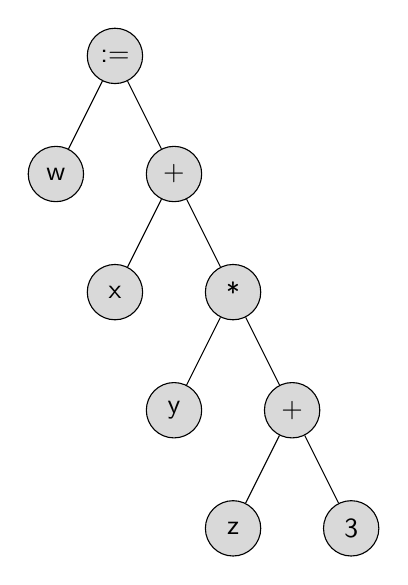
\begin{tikzpicture}
    \node[vertex]
    {:=}
        child {
            node[vertex] {w}
        } child {
            node[vertex] {+}
            child { node[vertex] {x} }
            child {
                node[vertex] {*}
                child { node[vertex] {y} }
                child {
                    node[vertex] {+}
                    child { node[vertex] {z} }
                    child { node[vertex] {3} }
                }
            }
        }
    ;
\end{tikzpicture} \\
\end{multicols}

\vspace{-8em}
\section{Generating Three-Address Code (3AC) from AST}
L-value := R-value
\begin{description}
  \item [L-values]: addresses which can be stored to or loaded from
  \item [R-values]: data (often loaded from addresses)
\end{description} \ \\
  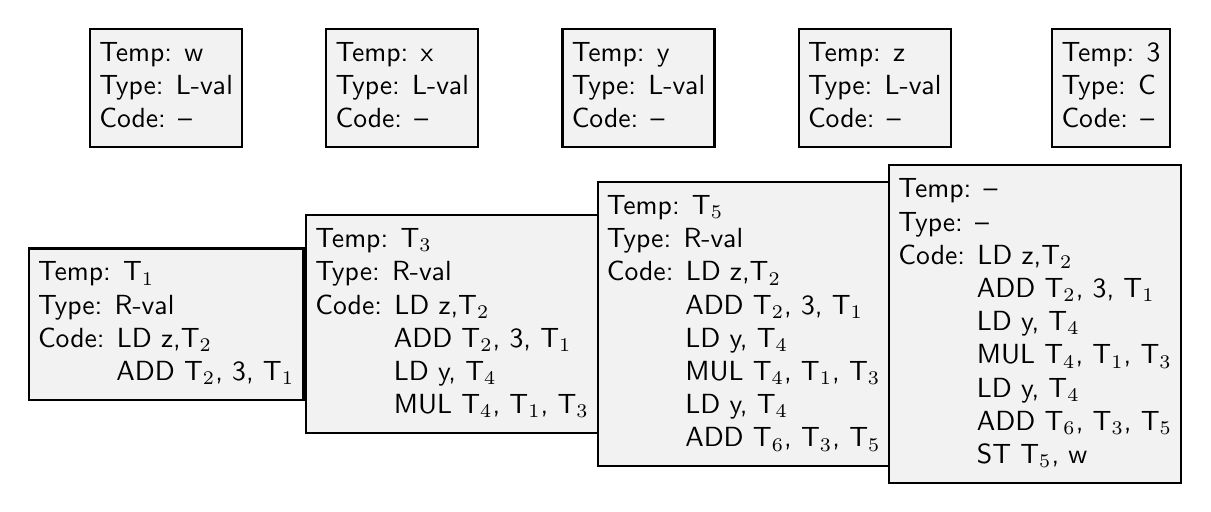
\begin{tikzpicture}
    \node[state, shape=rectangle] (0) {
    \makecell[l] {
    Temp: w \\
    Type: L-val \\
    Code: --
    }};
    \node[state, shape=rectangle, right of=0] (1) {
    \makecell[l] {
    Temp: x \\
    Type: L-val \\
    Code: --
    }};
    \node[state, shape=rectangle, right of=1] (2) {
    \makecell[l] {
    Temp: y \\
    Type: L-val \\
    Code: --
    }};
    \node[state, shape=rectangle, right of=2] (3) {
    \makecell[l] {
    Temp: z \\
    Type: L-val \\
    Code: --
    }};
    \node[state, shape=rectangle, right of=3] (4) {
    \makecell[l] {
    Temp: 3 \\
    Type: C \\
    Code: --
    }};
    \node[state, shape=rectangle, below of=0] (4) {
    \makecell[l] {
    Temp: T$_1$ \\
    Type: R-val \\
    Code: LD z,T$_2$ \\
    \hspace{2.5em} ADD T$_2$, 3, T$_1$
    }};
    \node[state, shape=rectangle, right of=4, xshift=18pt] (5) {
    \makecell[l] {
    Temp: T$_3$ \\
    Type: R-val \\
    Code: LD z,T$_2$ \\
    \hspace{2.5em} ADD T$_2$, 3, T$_1$ \\
    \hspace{2.5em} LD y, T$_4$ \\
    \hspace{2.5em} MUL T$_4$, T$_1$, T$_3$
    }};
    \node[state, shape=rectangle, right of=5, xshift=20pt] (6) {
    \makecell[l] {
    Temp: T$_5$ \\
    Type: R-val \\
    Code: LD z,T$_2$ \\
    \hspace{2.5em} ADD T$_2$, 3, T$_1$ \\
    \hspace{2.5em} LD y, T$_4$ \\
    \hspace{2.5em} MUL T$_4$, T$_1$, T$_3$ \\
    \hspace{2.5em} LD y, T$_4$ \\
    \hspace{2.5em} ADD T$_6$, T$_3$, T$_5$
    }};
    \node[state, shape=rectangle, right of=6, xshift=20pt] (7) {
    \makecell[l] {
    Temp: -- \\
    Type: -- \\
    Code: LD z,T$_2$ \\
    \hspace{2.5em} ADD T$_2$, 3, T$_1$ \\
    \hspace{2.5em} LD y, T$_4$ \\
    \hspace{2.5em} MUL T$_4$, T$_1$, T$_3$ \\
    \hspace{2.5em} LD y, T$_4$ \\
    \hspace{2.5em} ADD T$_6$, T$_3$, T$_5$ \\
    \hspace{2.5em} ST T$_5$, w
    }};
  \end{tikzpicture}


\section{In Class Quiz 7 - Slide 51}
\vspace{-1em}
\begin{multicols}{2}
Draw the AST for \textbfb{ x := z + 3}. What is the order of nodes visited when performing post-order traversal? \\
Post Order: \textbf{x, z, 3, +, :=} \\
  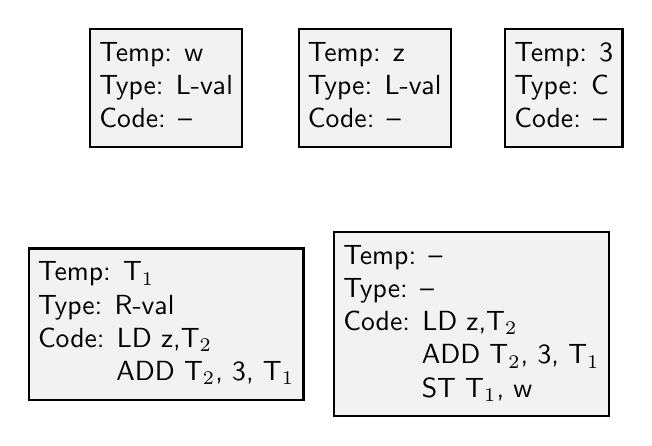
\begin{tikzpicture}
    \node[state, shape=rectangle] (0) {
    \makecell[l] {
    Temp: w \\
    Type: L-val \\
    Code: --
    }};
    \node[state, shape=rectangle, right of=0, xshift=-10pt] (1) {
    \makecell[l] {
    Temp: z \\
    Type: L-val \\
    Code: --
    }};
    \node[state, shape=rectangle, right of=1, xshift=-17pt] (2) {
    \makecell[l] {
    Temp: 3 \\
    Type: C \\
    Code: --
    }};
    \node[state, shape=rectangle, below of=0] (3) {
    \makecell[l] {
    Temp: T$_1$ \\
    Type: R-val \\
    Code: LD z,T$_2$ \\
    \hspace{2.5em} ADD T$_2$, 3, T$_1$
    }};
    \node[state, shape=rectangle, right of=3, xshift=25pt] (4) {
    \makecell[l] {
    Temp: -- \\
    Type: -- \\
    Code: LD z,T$_2$ \\
    \hspace{2.5em} ADD T$_2$, 3, T$_1$ \\
    \hspace{2.5em} ST T$_1$, w
    }};
  \end{tikzpicture}
\end{multicols}
\vspace{-12em}
\indent \hspace{10em}
  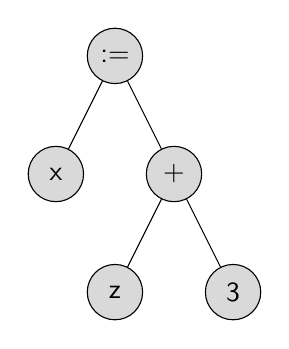
\begin{tikzpicture}
    \node[vertex]
    {:=}
        child {
            node[vertex] {x}
        } child {
            node[vertex] {+}
            child { node[vertex] {z} }
            child { node[vertex] {3} }
        }
    ;
  \end{tikzpicture}

\section{In Class Quiz 8 - Slide 52}
Draw the AST for \textbfb{x := z + 3}. Assume you perform post-order traversal
on this AST to generate code. How many lines of code are included in
the data object for the root node? \textbf{3} Lines of code


\chapter{Semantic Actions for Control Structures}
\section{Generate 3AC for If-elseif}
\vspace{-1em}
\begin{multicols}{2}
If-elseif statement: \\
\textr{if <bool\_expr\_1>} \\
\indent \textr{<stmt\_list\_1>} \\
\textb{else if <bool\_expr\_2>} \\
\indent \textb{<stmt\_list\_2>} \\
\textp{else} \\
\indent \textp{<stmt\_list\_3>} \\
\textg{Endif}
\section{In Class Quiz 1 - Slide 9}
\vspace{.5em}
Generate 3AC for the given if-elseif statement.
How many unconditional jumps and labels are included? \\
\textbf{2 jumps, 3 labels}
  \vfill\columnbreak
Generated assembly code: \\
\indent \textr{<code for bool\_expr\_1>} \\
\indent \textr{j<!op> ELSE\_1} \\
\indent \textr{<code for stmt\_list\_1>} \\
\indent \textr{jmp OUT\_1} \\
\textb{ELSE\_1:} \\
\indent \textb{<code for bool\_expr\_2>} \\
\indent \textb{j<!op> ELSE\_2} \\
\indent \textb{<code for stmt\_list\_2>} \\
\indent \textb{jmp OUT\_2} \\
\textp{ELSE\_2:} \\
\indent \textp{<code for stmt\_list\_3>} \\
\textg{OUT\_1:}
\end{multicols}


\section{Generate 3AC for While Loops}
\vspace{-1em}
\begin{multicols}{2}
while \textr{<bool\_expr>} \\
\indent \textb{<stmt\_list>} \\
endwhile;
\section{In Class Quiz 2 - Slide 14}
\vspace{1em}
In the previous While loop, what is the 3AC \\ 
for a \textit{break} statement? \textbf{jmp OUT}
  \vfill\columnbreak
LOOP: \\
\indent \textr{<bool\_expr>} \\
\indent j<!op> OUT \\
\indent \textb{<stmt\_list>} \\
\indent jmp LOOP \\
OUT:
\end{multicols}

\section{Generate 3AC for For Loops}
\vspace{-1em}
\begin{multicols}{2}
for (\textr{<init\_stmt>};\textb{<bool\_expr>};\textg{<incr\_stmt>}) \\
\indent \textp{<stmt\_list>} \\
end
\section{In Class Quiz 3 - Slide 19}
In the previous For loop, what is the 3AC \\
for a \textit{continue} statement?
\textbf{jmp INCR}
  \vfill\columnbreak
\indent \textr{<init\_stmt>} \\
LOOP: \\
\indent \textb{<bool\_expr>} \\
\indent j<!op> OUT \\
\indent \textp{<stmt\_list>} \\
INCR: \\
\indent \textg{<incr\_stmt>} \\
\indent jmp LOOP \\
OUT:
\end{multicols}

\section{Generate 3AC for Switch Statements}
\vspace{-1em}
\begin{multicols}{2}
switch (<expr>) \\
\indent case <const\_list>: <stmt\_list> \\
\indent case <const\_list>: <stmt\_list> \\
\indent ... \\
\indent default: <stmt\_list> \\
end
  \vfill\columnbreak
\indent <expr> \\
\indent <code for jump table> \\
LABEL0: \\
\indent <stmt\_list> \\
LABEL1: \\
\indent <stmt\_list> \\
\indent ... \\
DEFAULT: \\
\indent <stmt\_list> \\
OUT:
\end{multicols}


\end{document}
